\documentclass[11pt,letterpaper]{article}
\usepackage[lmargin=1in,rmargin=1in,tmargin=1in,bmargin=1in]{geometry}

% -------------------
% Packages
% -------------------
\usepackage{
	amsmath,			% Math Environments
	amssymb,			% Extended Symbols
	enumerate,		    % Enumerate Environments
	graphicx,			% Include Images
	lastpage,			% Reference Lastpage
	multicol,			% Use Multi-columns
	multirow			% Use Multi-rows
}
\graphicspath{ {./Images/} }


% -------------------
% Font
% -------------------
\usepackage[T1]{fontenc}
\usepackage{charter}


% -------------------
% Heading Commands
% -------------------
\newcommand{\class}{EECS 16ML}
\newcommand{\term}{Fall 2020}
\newcommand{\instructor}{Team RAAAK}
\newcommand{\head}[2]{%
\thispagestyle{empty}
\vspace*{-0.5in}
\noindent\begin{tabular*}{\textwidth}{l @{\extracolsep{\fill}} r @{\extracolsep{6pt}} l}
	\textbf{Quiz Topic: Outlier Removal via OMP} \\
	\textbf{\class:\; \term} & & \\
	\textbf{\instructor}
\end{tabular*} \\
\rule[2ex]{\textwidth}{2pt} %
}


% -------------------
% Commands
% -------------------
\newcommand{\prob}{\noindent\textbf{Problem. }}
\newcounter{problem}
\newcommand{\problem}{
	\stepcounter{problem}%
	\noindent \textbf{Part \theproblem. }%
}
\newcommand{\pointproblem}[1]{
	\stepcounter{problem}%
	\noindent \textbf{Part \theproblem.} (#1 points)\,%
}
\newcommand{\pspace}{\par\vspace{\baselineskip}}
\newcommand{\ds}{\displaystyle}


% -------------------
% Header & Footer
% -------------------
\usepackage{fancyhdr}

\fancypagestyle{pages}{
	%Headers
	\fancyhead[L]{}
	\fancyhead[C]{}
	\fancyhead[R]{}
\renewcommand{\headrulewidth}{0pt}
	%Footers
	\fancyfoot[L]{}
	\fancyfoot[C]{}
	\fancyfoot[R]{}
\renewcommand{\footrulewidth}{0.0pt}
}
\headheight=0pt
\footskip=14pt

\pagestyle{pages}


% -------------------
% Content
% -------------------
\begin{document}
\textbf{EECS 16ML Quiz: Outlier Removal via OMP} \pspace


% Question 1
\problem Use the following matrix equation setup to run OMP for two iterations. Please box the intermediate and final residuals as well as the two components identified to have non-zero entries.

\begin{equation*}
    \begin{bmatrix}
        \boldsymbol{A} & \boldsymbol{I}
    \end{bmatrix}\begin{bmatrix}
        \vec{x} \\
        \vec{\epsilon}
    \end{bmatrix}
     = \vec{y} \Rightarrow
    \begin{bmatrix}
         1 & 1 & 0 & 1 & 1 & 0 & 0 & 0 \\
         1 & 1 & 0 & 0 & 0 & 1 & 0 & 0 \\
         1 & 0 & 1 & 1 & 0 & 0 & 1 & 0 \\
         1 & 0 & 1 & 0 & 0 & 0 & 0 & 1
    \end{bmatrix}
    \begin{bmatrix}
         a \\ b \\ c \\ d \\ e \\ f \\ g \\ h
    \end{bmatrix}
    =\begin{bmatrix}
         2 \\ 0 \\ 2 \\ 1
    \end{bmatrix}
\end{equation*}

\begin{enumerate}
    \item \textbf{Solution}: Iteration 1 Component:
        \begin{equation*}
            \langle\vec{y},\vec{c_{1}}\rangle = 5,        \langle\vec{y},\vec{c_{2}}\rangle = 2,
            \langle\vec{y},\vec{c_{3}}\rangle = 3,
            \langle\vec{y},\vec{c_{4}}\rangle = 4,
            \langle\vec{y},\vec{c_{5}}\rangle = 2,
            \langle\vec{y},\vec{c_{6}}\rangle = 0,
            \langle\vec{y},\vec{c_{7}}\rangle = 2,
            \langle\vec{y},\vec{c_{8}}\rangle = 1
        \end{equation*}
        We first pick the vector that "explains" the largest component of $\vec{y}$, which translates to picking the vector with the largest dot product from above, $\vec{c_{1}}$.
	\item \textbf{Solution}: Iteration 1 Residual: \\
	    We then calculate $\vec{y_{1}}$, the component of $\vec{y}$ that is explained by $\vec{c_{1}}$, using least squares with $\vec{c_{1}}$ and $\vec{y}$. This is followed by calculating the residual, $\vec{r_{1}}$, that represents the leftover component of $\vec{y}$ not accounted for by $\vec{y_{1}}$.
	    \begin{equation*}
            \vec{y_{1}} = \vec{c_{1}}(\vec{c_{1}}^T\vec{c_{1}})^{-1}\vec{c_{1}}^T\vec{y} = \begin{bmatrix}
                 1 \\ 1 \\ 1 \\ 1
            \end{bmatrix} *(\frac{1}{4}) * 5
            = \begin{bmatrix}
                 \frac{5}{4} \\ \frac{5}{4} \\ \frac{5}{4} \\ \frac{5}{4}
            \end{bmatrix} \Rightarrow
            \vec{r_{1}} = \vec{y} - \vec{y_{1}} = 
            \begin{bmatrix}
                \frac{3}{4} \\ -\frac{5}{4} \\ \frac{3}{4} \\ -\frac{1}{4} 
            \end{bmatrix}
        \end{equation*}
	\item \textbf{Solution}: Iteration 2 Component: \\
	    We now repeat the process, using $\vec{r_{1}}$ to compute dot products with rather than the original vector $\vec{y}$.
        \begin{equation*}
            \langle\vec{r_{1}},\vec{c_{1}}\rangle = 5,        \langle\vec{r_{1}},\vec{c_{2}}\rangle = -\frac{2}{4},
            \langle\vec{r_{1}},\vec{c_{3}}\rangle = \frac{2}{4},
            \langle\vec{r_{1}},\vec{c_{4}}\rangle = \frac{6}{4},
            \langle\vec{r_{1}},\vec{c_{5}}\rangle = \frac{3}{4},
            \langle\vec{r_{1}},\vec{c_{6}}\rangle = -\frac{5}{4},
            \langle\vec{r_{1}},\vec{c_{7}}\rangle = \frac{3}{4},
            \langle\vec{r_{1}},\vec{c_{8}}\rangle = -\frac{1}{4}
        \end{equation*}
        We choose to proceed with $\vec{c_{4}}$.
	\item \textbf{Solution}: Iteration 2 Residual: \\
	    We now calculate $\vec{y_{2}}$, the amount of $\vec{y}$ accounted for by both $\vec{c_{1}}$ and $\vec{c_{4}}$, and the resulting residual, $\vec{r_{2}}$. For notational convenience, we define the following:
        \begin{equation*}
            \boldsymbol{A_{2}} = \begin{bmatrix}
                \vec{c_{1}} && \vec{c_{4}}
            \end{bmatrix} \Rightarrow
            \vec{y_{2}} = \boldsymbol{A_{2}}(\boldsymbol{A_{2}}^T\boldsymbol{A_{2}})^{-1}\boldsymbol{A_{2}}^T\vec{y} = \begin{bmatrix}
                2 \\ \frac{1}{2} \\ 2 \\ \frac{1}{2}
            \end{bmatrix} \Rightarrow
            \vec{r_{2}} = \vec{y} - \vec{y_{2}} = \begin{bmatrix}
                0 \\ -\frac{1}{2} \\ 0 \\ \frac{1}{2}
            \end{bmatrix} 
        \end{equation*}
	    
\end{enumerate} 

\newpage
% Question 2
\problem Ignore the calculations done in the first problem. Suppose that a genie ran OMP for the problem above and told you the following about the sparse solution: %\vfill
\begin{equation*}
    \vec{x} = \begin{bmatrix}
        \frac{1}{2} \\ 1 \\ -\frac{1}{2} \\ 1
    \end{bmatrix}, \vec{\epsilon} = \begin{bmatrix}
        0 \\ 10 \\ -\frac{1}{2} \\ 0
    \end{bmatrix}
\end{equation*}
Interpret the results by identifying the outlier(s). Provide justification/explanation. \\

\textbf{Solution}: \\
The first and last points from the data matrix have a "0" as their corresponding entry in $\vec{\epsilon}$, meaning that these two point are aligned and reflect the presumed pattern. However, the second point has a very large entry in $\vec{\epsilon}$, leading us to call it an outlier. The third point is more ambiguous and could be classified as an outlier for having a non-zero entry or be classified a non-outlier, since there are so few points that an entry with such a small magnitude compared to the other outlier can be ignored. Either answer would be marked correct for the third point as long as the justification suffices.

\vspace{1cm}

% Question 3
\problem In each of the three parts below, describe a potential stopping condition discussed in this course for OMP. In addition to naming the stopping condition, describe potential (dis)advantages and/or use cases. The order you list them in does not matter.
	\begin{enumerate}
	\item \textbf{Solution}: Stopping Condition 1:
	    \begin{enumerate}[(a)]
	        \item Description: One potential stopping condition is to stop after running $k$ iterations, where $k$ is the parameter passed into the OMP function representing either the number of outliers.
	        \item Use Cases: An apparent disadvantage to this stopping condition is that it can only be used when the user has absolute knowledge or an approximate estimate about the number of outliers in the dataset, an assumption that is not typically met. In the case that the user does not have adequate confidence in their estimate of the number of outliers, $k$ could be treated as a hyperparmeter that is tuned for optimal performance using the validation set. 
	    \end{enumerate}
	\item \textbf{Solution}: Stopping Condition 2:
	    \begin{enumerate}[(a)]
	        \item Description: The next stopping condition is when the residual falls below a specific threshold value. This threshold value would be passed into the OMP function and is typically treated as a hyperparameter.
	        \item Use Cases: This is more generalizable than the previous stopping condition because the number of outliers is likely dependent on the size of the dataset, while the threshold value can be tuned and then re-used for a datasets of varying sizes. This stopping condition helps to prevent OMP from aiming towards an absolute 0 residual, which is very unlikely in real-world datasets. For most purposes, as long as the residual is sufficiently small, we consider all the outliers to have been identified.
	    \end{enumerate}
	\item \textbf{Solution}: Stopping Condition 3:
	    \begin{enumerate}[(a)]
	        \item Description: The last stopping condition is to stop once there are only two non-outlier points left in the set.
	        \item Use Cases: This stopping condition is more of a fail-safe rather than the primary stopping condition, because two points is the minimum number of points to actually establish a linear relationship, the simplest mathematical pattern. OMP implementations usually rely on a more controllable stopping condition, such as one of the two above, because, as you can imagin, most real-world applications probably do not want all but two of the points in the dataset to be classified as outliers.
	    \end{enumerate}
	\end{enumerate}

\vspace{1cm}

\problem Observe the graph below and describe what happens to the training and validation errors in the each of the two labeled regions.
\begin{figure}[!h]
  \centering
  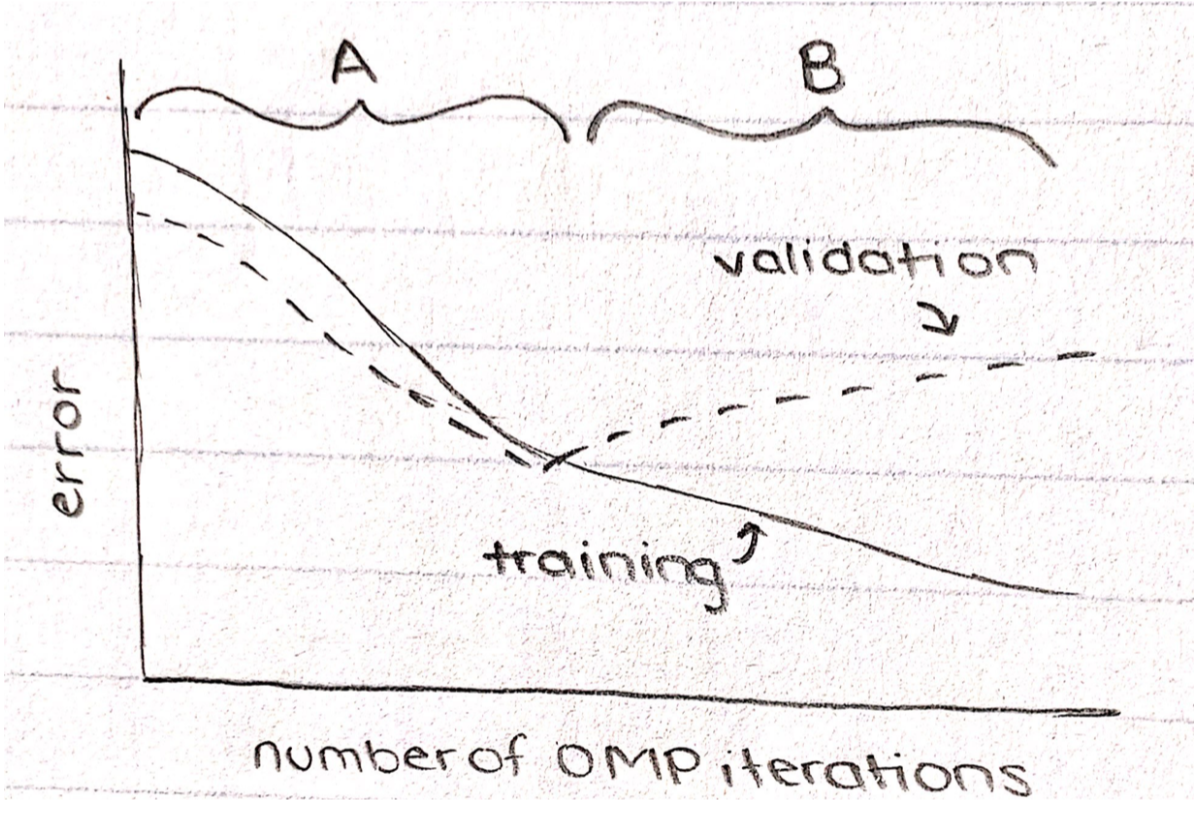
\includegraphics[scale=0.3]{graph}
\end{figure}
    \begin{enumerate}
        \item \textbf{Solution}: Region A, Training Error: \\
            In this region, the training error decreases as the initial outliers are identified and the linear pattern is more strongly observed in the remaining points. 
        \item \textbf{Solution}: Region A, Validation Error:
            In this region, like for the training error, elimination of outliers has produced a model that represents a majority of the points in the validation set. 
        \item \textbf{Solution}: Region B, Training Error:
            This is essentially when the model ends up discarding points that are not actually outliers due to the $k$ parameter being too high. More and more points are observed to be outliers, allowing the model to fit to a decreasing number of points that happen to be highly correlated.
        \item \textbf{Solution}: Region B, Validation Error:
            Because normal points are being classified as outliers in training, the validation error increases in this region due to the model not encapsulating the general pattern of the overall dataset. This reflects the effect of not properly tuning the $k$ hyperparameter in on the test error.
    \end{enumerate}



\end{document}			